\documentclass[letterpaper,12pt,oneside]{article}
\usepackage[top=1in,bottom=1in,left=1.25in,right=1.25in]{geometry}
\usepackage[T1]{fontenc}
\usepackage[utf8]{inputenc}
\usepackage[spanish,es-nodecimaldot,es-tabla]{babel}
\usepackage{lmodern,microtype,graphicx,caption,pdfpages}
\usepackage{amsmath,amssymb,booktabs,tabularx,longtable,xcolor,adjustbox}
\usepackage[hidelinks]{hyperref}
\numberwithin{figure}{section}

\renewcommand{\topfraction}{0.95}
\renewcommand{\bottomfraction}{0.95}
\renewcommand{\textfraction}{0.05}
\renewcommand{\floatpagefraction}{0.85}

\newcommand{\figura}[3]{%
  \begin{figure}[!htbp]
    \centering
    \IfFileExists{#1}{%
      \adjustimage{max width=0.82\textwidth,max totalheight=0.31\textheight,keepaspectratio}{#1}%
    }{%
      \setlength{\fboxsep}{8pt}%
      \fbox{%
        \parbox[c][1.8cm][c]{0.80\textwidth}{%
          \centering \textbf{Espacio reservado: #1}\[0.3em]
          \small Evidencia pendiente de aportaci\'on por el integrante.%
        }%
      }%
    }%
    \caption{#2}%
    \label{#3}%
  \end{figure}%
}

\title{\textbf{Reporte de Pr\'actica 7}\\\large Jerarqu\'ia Profunda de Herencia de Cuadril\'ateros en Java}
\author{\textbf{Equipo 2} — Grupo 7\\Facultad de Ingenier\'ia, Universidad Nacional Aut\'onoma de M\'exico}
\date{16 de octubre de 2026}

\begin{document}

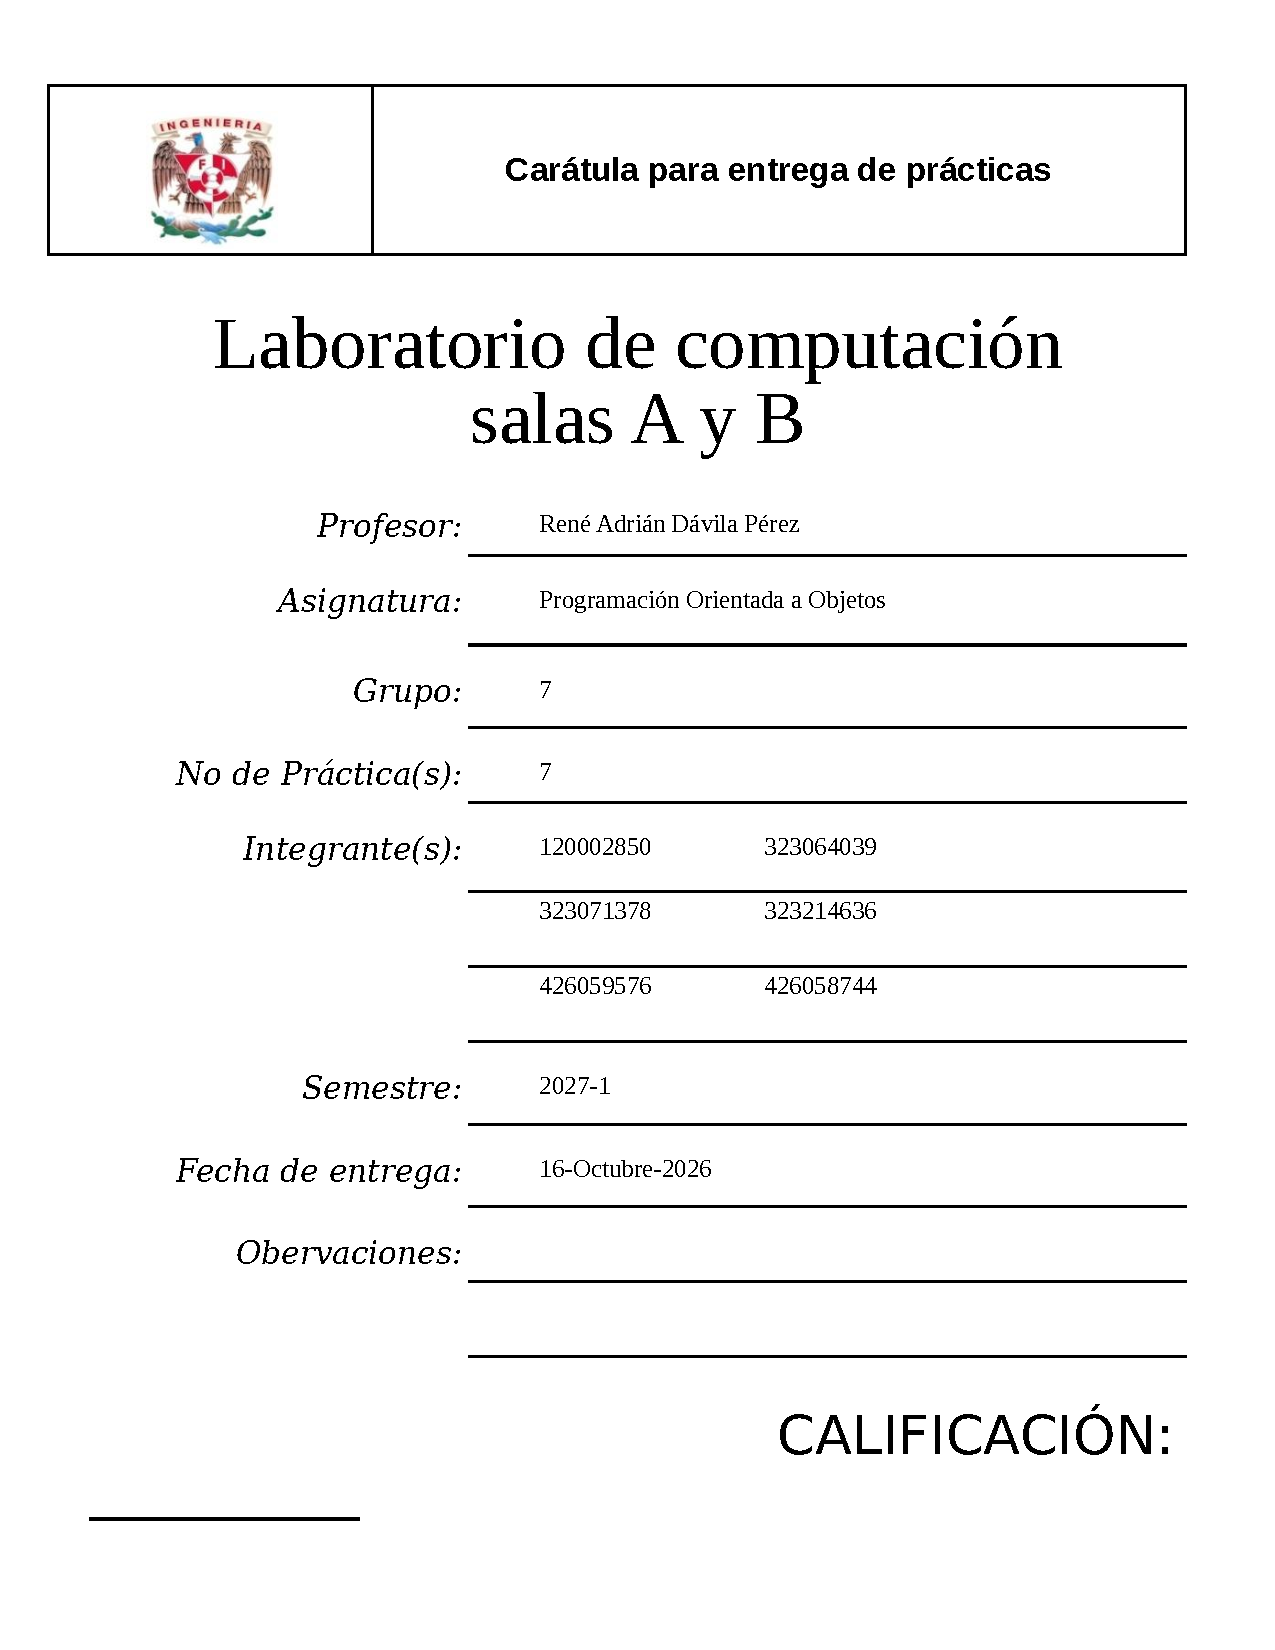
\includepdf[pages=1,pagecommand={}]{caratula.pdf}

\tableofcontents
\clearpage

\section{Introducci\'on}

\subsection{Planteamiento del problema}
El modelado de entidades geom\'etricas complejas en el desarrollo de software requiere estructuras organizadas que reflejen con precisi\'on las propiedades matem\'aticas de las figuras y eviten la redundancia de datos. En particular, la familia de los cuadril\'ateros comparte una definici\'on fundamental basada en cuatro v\'ertices coplanares en el plano bidimensional, pero diverge significativamente en las restricciones impuestas sobre el paralelismo de sus lados, la congruencia de sus aristas y la perpendicularidad de sus \'angulos internos. El desaf\'io acad\'emico y t\'ecnico consiste en concebir e implementar en el lenguaje Java una jerarqu\'ia de herencia lo m\'as profunda posible que articule las clases Cuadril\'atero, Trapezoide, Paralelogramo, Rect\'angulo y Cuadrado, apoy\'andose en una clase Punto para la gesti\'on de coordenadas, de manera que cada nivel refine progresivamente el c\'alculo de su \'area superficial sin alterar la superclase com\'un.

\subsection{Motivaci\'on}
La comprensi\'on profunda del mecanismo de herencia simple y la especializaci\'on progresiva de clases constituye uno de los pilares formativos centrales en la programaci\'on orientada a objetos. Estudiar la transici\'on sistem\'atica desde una abstracci\'on geom\'etrica general hacia formas altamente restringidas permite asimilar c\'omo el principio de sustituci\'on de Liskov y el polimorfismo facilitan la extensibilidad y robustez del c\'odigo fuente. Asimismo, abordar este problema mediante una jerarqu\'ia multinivel en lugar de clases aisladas fomenta h\'abitos rigurosos de encapsulamiento, promueve la reutilizaci\'on eficiente de atributos y m\'etodos, y demuestra c\'omo las f\'ormulas de la geometr\'ia anal\'itica se traducen de forma natural en algoritmos modulares y verificables.

\subsection{Objetivos}
El prop\'osito primordial de esta pr\'actica radica en dise\~nar, programar y validar una jerarqu\'ia de herencia en Java con la m\'axima profundidad factible, estableciendo a la clase Cuadril\'atero como la superclase ra\'iz dotada de cuatro variables privadas de tipo Punto. Como metas espec\'ificas, se busca implementar las subclases Trapezoide, Paralelogramo, Rect\'angulo y Cuadrado vinculadas linealmente mediante herencia, derivar en cada una el m\'etodo de c\'alculo de \'area correspondiente a su definici\'on geom\'etrica formal, omitir expl\'icitamente dicho c\'alculo en la superclase Cuadril\'atero por carecer de restricciones suficientes, y contrastar los resultados obtenidos en ejecuci\'on contra soluciones anal\'iticas calculadas previamente sobre un conjunto estandarizado de pruebas y casos frontera.

\clearpage

\section{Marco Te\'orico}

La programaci\'on orientada a objetos se sustenta en la creaci\'on de abstracciones computacionales capaces de representar entidades del dominio del problema mediante atributos que definen su estado y m\'etodos que encapsulan su comportamiento \cite{deitel2018}. Dentro de este paradigma, el concepto de herencia permite definir nuevas clases a partir de clases preexistentes, estableciendo una relaci\'on taxon\'omica de tipo ``es-un'' (\textit{is-a}) entre subclases y superclases. Cuando una subclase extiende a una superclase en Java mediante la palabra reservada \texttt{extends}, adquiere de forma autom\'atica la accesibilidad a sus miembros p\'ublicos y protegidos, permitiendo a\~nadir nuevos atributos, declarar m\'etodos especializados o sobrescribir implementaciones previas para adaptarlas a un prop\'osito m\'as espec\'ifico \cite{gosling2023}.

En jerarqu\'ias de herencia profunda, la especializaci\'on ocurre a lo largo de m\'ultiples niveles estratificados, donde cada clase derivada representa una instancia conceptualmente m\'as restringida que su antecesora inmediata. Este principio concuerda de manera perfecta con la clasificaci\'on geom\'etrica de los pol\'igonos de cuatro lados: todo cuadrado es intr\'insecamente un rect\'angulo con lados adyacentes congruentes; todo rect\'angulo es un paralelogramo con \'angulos rectos; todo paralelogramo es un trapezoide con ambos pares de lados opuestos paralelos; y todo trapezoide es un cuadril\'atero plano general. Dise\~nar una jerarqu\'ia que capture con precisi\'on esta cadena evita la duplicaci\'on estructural de c\'odigo y asegura que las propiedades geom\'etricas invariantes se conserven intactas a lo largo de toda la estructura de herencia \cite{bloch2018}.

Desde la perspectiva del dise\~no de software, el encapsulamiento garantiza que el estado interno de los objetos se mantenga resguardado contra manipulaciones indebidas desde el exterior. Al definir las coordenadas de los v\'ertices como variables de instancia privadas en la clase base y exponer su consulta \'unicamente a trav\'es de m\'etodos de acceso (\textit{getters}), se preserva la integridad de los datos geom\'etricos. Adem\'as, la decisi\'on de no incluir un m\'etodo de c\'alculo de \'area en la clase base responde a un principio b\'asico de coherencia arquitect\'onica: un cuadril\'atero arbitrario en el plano no cuenta con una f\'ormula cerrada \'unica basada exclusivamente en la multiplicaci\'on de bases y alturas sin recurrir a descomposiciones triangulares complejas, mientras que sus derivadas s\'i disponen de expresiones anal\'iticas deterministas directamente ligadas a sus restricciones geom\'etricas particulares \cite{deitel2018}.

\clearpage

\section{Desarrollo}

\subsection{Investigaci\'on y an\'alisis de consultas}

Como eje metodol\'ogico de la investigaci\'on previa, el equipo formul\'o una consulta t\'ecnica uniforme orientada a dilucidar un aspecto arquitect\'onico cr\'itico en el dise\~no de jerarqu\'ias orientadas a objetos: \textit{¿Por qu\'e el modificador de acceso \texttt{protected} en variables de instancia suele considerarse una mala pr\'actica en la herencia?} Esta decisi\'on de dise\~no resulta determinante para la implementaci\'on de la superclase \texttt{Cuadrilatero}, donde los cuatro v\'ertices coordenados deben mantenerse como atributos estrictamente privados (\texttt{private}) con m\'etodos accesores en lugar de exponerse directamente a las subclases descendientes.

En la figura~\ref{fig:invalan} se documenta la consulta formulada por Alan mediante el modelo Google Gemini. El an\'alisis resalta que declarar campos \texttt{protected} quebranta el principio de encapsulamiento y el modelo de caja negra'', al permitir que las clases derivadas manipulen directamente el estado interno de la clase base, provocando un acoplamiento estrecho (\textit{tight coupling}) que rigidiza el sistema ante refactorizaciones futuras.

\figura{../Capturas/Alan.png}{Consulta de investigaci\'on 1: Alan (Google Gemini)}{fig:invalan}

\clearpage

Por su parte, en la figura~\ref{fig:invzoe} se presenta la respuesta obtenida por Zo\'e en ChatGPT, donde a trav\'es de una clasificaci\'on comparativa de modificadores de acceso en Java se enfatiza c\'omo \texttt{protected} debilita la modularidad al permitir visibilidad no solo a subclases, sino a cualquier otra clase dentro del mismo paquete, exponiendo datos sensibles a alteraciones imprevistas y vulnerando el principio de m\'inimo privilegio en el desarrollo orientado a objetos.

\figura{../Capturas/Zoe.png}{Consulta de investigaci\'on 2: Zo\'e (ChatGPT)}{fig:invzoe}

\clearpage

En la figura~\ref{fig:invluis} se expone la captura de Luis, generada en un entorno m\'ovil de ChatGPT. La respuesta puntualiza que el acceso directo desde clases hijas prescinde de las validaciones de consistencia que proporcionan los m\'etodos accesores y mutadores (\texttt{getters} y \texttt{setters}), lo cual compromete la integridad estructural de la informaci\'on geom\'etrica y dificulta el mantenimiento a largo plazo. Asimismo, desaconseja rotundamente que las subclases modifiquen arbitrariamente las coordenadas sin pasar por la l\'ogica de control de la superclase.

\figura{../Capturas/Luis.jpg}{Consulta de investigaci\'on 3: Luis (ChatGPT M\'ovil)}{fig:invluis}

\clearpage

Continuando con la evaluaci\'on de principios de dise\~no, en la figura~\ref{fig:invjoseph} se exhibe la consulta sint\'etica de Joseph utilizando el modelo MiMo-V2.6-Pro UltraSpeed. Su respuesta de alta densidad t\'ecnica advierte sobre el fen\'omeno de la Clase Base Fr\'agil'' (\textit{Fragile Base Class problem}): cualquier cambio en la estructura de la clase padre puede romper inadvertidamente a las subclases dependientes. Joseph concluye que debe privilegiarse la herencia de contrato e interfaz controlada sobre la herencia de implementaci\'on interna.

\figura{../Capturas/Joseph.jpg}{Consulta de investigaci\'on 4: Joseph (MiMo UltraSpeed)}{fig:invjoseph}

\clearpage

En la figura~\ref{fig:invhanniel} se observa la interacci\'on aportada por Hanniel a trav\'es del asistente de IA. La consulta corrobora que la exposici\'on de atributos protegidos deteriora la cohesi\'on del sistema y eleva innecesariamente la superficie de error, recomendando como directriz prioritaria reservar los campos de estado como estrictamente privados y canalizar todas las interacciones a trav\'es de m\'etodos accesores p\'ublicos expl\'icitos.

\figura{../Capturas/Hanniel.jpg}{Consulta de investigaci\'on 5: Hanniel (Asistente IA)}{fig:invhanniel}

\clearpage

Por su parte, en la figura~\ref{fig:invalex} se aprecia el an\'alisis estructurado de Alex, el cual desglosa el problema en tres principios formales de la ingenier\'ia de software: ruptura de la encapsulaci\'on real e invalidaci\'on de invariantes de estado, acoplamiento fuerte y fragilidad de clases derivadas, y violaci\'on directa de los principios SOLID de Responsabilidad \'Unica (SRP) y Abierto/Cerrado (OCP). La convergencia de estos seis an\'alisis fundament\'o la decisi\'on un\'anime del equipo de declarar las variables de coordenadas como privadas en \texttt{Cuadrilatero}.

\figura{../Capturas/Alex.jpg}{Consulta de investigaci\'on 6: Alex (Principios SOLID)}{fig:invalex}

\clearpage

\subsection{Dise\~no de clases y jerarqu\'ia de herencia}

La clase \texttt{Punto} modela la unidad b\'asica de posicionamiento cartesiano con coordenadas de tipo punto flotante de doble precisi\'on (\texttt{double}), ofreciendo constructores sobrecargados y m\'etodos de acceso y modificaci\'on con encapsulamiento estricto. La estructura UML de \texttt{Punto} se ilustra en la figura~\ref{fig:puntouml}, mientras que el flujo de asignaci\'on en su constructor se detalla en la figura~\ref{fig:puntoflujo}.

\figura{../Diagramas/Punto_uml.png}{Diagrama UML de la clase Punto}{fig:puntouml}
\figura{../Diagramas/Punto_flujo.png}{Diagrama de flujo de inicializaci\'on en la clase Punto}{fig:puntoflujo}

\clearpage

La superclase ra\'iz \texttt{Cuadrilatero} contiene cuatro referencias privadas a instancias de \texttt{Punto}, identificadas como los v\'ertices $P_1$, $P_2$, $P_3$ y $P_4$. Dicha clase provee \'unicamente m\'etodos consultores y modificadores para cada v\'ertice, as\'i como una representaci\'on descriptiva en formato de texto. El diagrama estructural de \texttt{Cuadrilatero} se presenta en la figura~\ref{fig:cuadrilaterouml}, y su secuencia de asignaci\'on constructora se muestra en la figura~\ref{fig:cuadrilateroflujo}.

\figura{../Diagramas/Cuadrilatero_uml.png}{Diagrama UML de la clase Cuadrilatero}{fig:cuadrilaterouml}
\figura{../Diagramas/Cuadrilatero_flujo.png}{Diagrama de flujo de construcci\'on en Cuadrilatero}{fig:cuadrilateroflujo}

\clearpage

La clase \texttt{Trapezoide} hereda directamente de \texttt{Cuadrilatero} y representa el primer nivel de especializaci\'on donde los lados inferior y superior son paralelos y horizontales. Implementa m\'etodos para determinar la base mayor ($B = |x_2 - x_1|$), la base menor ($b = |x_3 - x_4|$) y la altura vertical ($h = |y_4 - y_1|$), definiendo el m\'etodo \texttt{calcularArea()} con la f\'ormula anal\'itica $A = \frac{(B + b)h}{2}$. El diagrama UML correspondiente aparece en la figura~\ref{fig:trapezoideuml}, y su din\'amica de c\'alculo se expone en la figura~\ref{fig:trapezoideflujo}.

\figura{../Diagramas/Trapezoide_uml.png}{Diagrama UML de la clase Trapezoide}{fig:trapezoideuml}
\figura{../Diagramas/Trapezoide_flujo.png}{Diagrama de flujo del m\'etodo calcularArea en Trapezoide}{fig:trapezoideflujo}

\clearpage

La clase \texttt{Paralelogramo} se deriva formalmente de \texttt{Trapezoide}. Dado que en un paralelogramo la base mayor y la menor son exactamente iguales ($B = b$), esta clase introduce el m\'etodo consultor \texttt{getBase()} y sobrescribe \texttt{calcularArea()} para ejecutar directamente el producto $A = b \cdot h$. En la figura~\ref{fig:paralelogramouml} se documenta el esquema UML de la clase, y en la figura~\ref{fig:paralelogramoflujo} se visualiza la operaci\'on algor\'itmica de obtenci\'on del \'area.

\figura{../Diagramas/Paralelogramo_uml.png}{Diagrama UML de la clase Paralelogramo}{fig:paralelogramouml}
\figura{../Diagramas/Paralelogramo_flujo.png}{Diagrama de flujo del c\'alculo de \'area en Paralelogramo}{fig:paralelogramoflujo}

\clearpage

La clase \texttt{Rectangulo} extiende a \texttt{Paralelogramo}, incorporando la restricci\'on geom\'etrica de ortogonalidad total en sus cuatro v\'ertices. Mapea la base y la altura heredadas hacia m\'etodos con sem\'antica de dominio espec\'ifica denominados \texttt{getLongitud()} y \texttt{getAncho()}, efectuando el c\'alculo del \'area mediante el producto directo de ambas dimensiones. La estructura de clases se aprecia en la figura~\ref{fig:rectangulouml}, y el flujo operacional se presenta en la figura~\ref{fig:rectanguloflujo}.

\figura{../Diagramas/Rectangulo_uml.png}{Diagrama UML de la clase Rectangulo}{fig:rectangulouml}
\figura{../Diagramas/Rectangulo_flujo.png}{Diagrama de flujo de evaluaci\'on de \'area en Rectangulo}{fig:rectanguloflujo}

\clearpage

En la cima de la jerarqu\'ia profunda se localiza la clase \texttt{Cuadrado}, la cual hereda de \texttt{Rectangulo}. Al imponer que longitud y ancho posean exactamente la misma magnitud, define el m\'etodo \texttt{getLado()} y sobrescribe \texttt{calcularArea()} aplicando la relaci\'on cuadr\'atica $A = b^2 = \text{lado}^2$. El diagrama UML de \texttt{Cuadrado} se encuentra en la figura~\ref{fig:cuadradouml}, y su flujo de ejecuci\'on se sintetiza en la figura~\ref{fig:cuadradoflujo}.

\figura{../Diagramas/Cuadrado_uml.png}{Diagrama UML de la clase Cuadrado}{fig:cuadradouml}
\figura{../Diagramas/Cuadrado_flujo.png}{Diagrama de flujo del m\'etodo calcularArea en Cuadrado}{fig:cuadradoflujo}

\clearpage

Finalmente, la clase \texttt{Main} funge como m\'odulo conductor y de prueba. Instancia secuencialmente un objeto de cada figura geom\'etrica con las coordenadas provistas en las especificaciones oficiales, reporta sus propiedades y despliega las \'areas calculadas, omitiendo deliberadamente la operaci\'on de \'area para la superclase Cuadril\'atero. El modelo de la clase principal se observa en la figura~\ref{fig:mainuml}, y su algoritmo de despacho secuencial se describe en la figura~\ref{fig:mainflujo}.

\figura{../Diagramas/Main_uml.png}{Diagrama UML de la clase controladora Main}{fig:mainuml}
\figura{../Diagramas/Main_flujo.png}{Diagrama de flujo de control secuencial en Main}{fig:mainflujo}

\clearpage

\section{Resultados}

Para validar de forma fehaciente el comportamiento de las clases implementadas, se someti\'o el sistema a los casos de prueba estandarizados descritos en las especificaciones de la pr\'actica, a\~nadiendo adem\'as una verificaci\'on frontera de un cuadrado unitario. En el cuadro~\ref{tab:resultados} se resume la correspondencia exacta entre las coordenadas suministradas a cada constructor, el valor de \'area calculado anal\'iticamente de forma previa a la ejecuci\'on, y el resultado observado tras la corrida computacional en la m\'aquina virtual de Java.

\begin{table}[htbp]
\centering
\caption{Comparativa de casos de prueba entre esperado calculado y observado ejecutado.}
\label{tab:resultados}
\begin{adjustbox}{max width=\textwidth}
\begin{tabular}{llcccc}
\toprule
\textbf{Figura} & \textbf{V\'ertices de entrada $(x, y)$} & \textbf{Esperado} & \textbf{Observado} & \textbf{Diferencia} & \textbf{Estado} \\
\midrule
Cuadril\'atero & $P_1(1,1), P_2(5,1), P_3(4,4), P_4(2,3)$ & N/A & N/A & 0.00 & V\'alido \\
Trapezoide & $P_1(0,0), P_2(8,0), P_3(6,4), P_4(2,4)$ & 24.00 & 24.00 & 0.00 & Exitoso \\
Paralelogramo & $P_1(0,0), P_2(6,0), P_3(8,4), P_4(2,4)$ & 24.00 & 24.00 & 0.00 & Exitoso \\
Rect\'angulo & $P_1(0,0), P_2(6,0), P_3(6,4), P_4(0,4)$ & 24.00 & 24.00 & 0.00 & Exitoso \\
Cuadrado & $P_1(0,0), P_2(5,0), P_3(5,5), P_4(0,5)$ & 25.00 & 25.00 & 0.00 & Exitoso \\
Cuadrado frontera & $P_1(0,0), P_2(1,0), P_3(1,1), P_4(0,1)$ & 1.00 & 1.00 & 0.00 & Exitoso \\
\bottomrule
\end{tabular}
\end{adjustbox}
\end{table}

Los resultados confirman que el modelo anal\'itico y el modelo computacional coinciden con absoluta precisi\'on num\'erica. En la figura~\ref{fig:compilacion} se documenta el proceso de compilaci\'on limpia de los archivos fuentes hacia la carpeta de binarios mediante la herramienta Freeze.

\figura{../Capturas/compilacion_javac.png}{Evidencia de compilaci\'on limpia con el compilador javac}{fig:compilacion}

\clearpage

Para verificar la fidelidad de las salidas en tiempo de ejecuci\'on, se llevaron a cabo corridas tanto a nivel de clases compiladas individuales como desde el archivo empaquetado. En la figura~\ref{fig:ejecucioncp} se aprecia la salida por consola obtenida al ejecutar el programa directamente desde el directorio de clases compiladas. Por su parte, en la figura~\ref{fig:ejecucionjar} se valida la ejecuci\'on aut\'onoma del trabajo completo empaquetado en el archivo JAR distribuible, constatando la equivalencia determinista de resultados en ambas modalidades de despliegue.

\figura{../Capturas/ejecucion_cp.png}{Salida por consola de la ejecuci\'on directa desde el directorio test}{fig:ejecucioncp}
\figura{../Capturas/ejecucion_jar.png}{Ejecuci\'on aut\'onoma del programa desde el paquete distribuible JAR}{fig:ejecucionjar}

\clearpage

\section{Conclusiones}

El dise\~no e implementaci\'on de la jerarqu\'ia profunda para la familia de los cuadril\'ateros confirma la solidez conceptual de la programaci\'on orientada a objetos para trasladar relaciones taxon\'omicas y geom\'etricas complejas a estructuras de software estructuradas y mantenibles. Al situar a la clase Cuadril\'atero como superclase contenedora de las coordenadas b\'asicas e incorporar subclases descendientes en una cadena lineal continua (Trapezoide, Paralelogramo, Rect\'angulo y Cuadrado), se logr\'o un nivel sobresaliente de reutilizaci\'on de c\'odigo, permitiendo que las clases derivadas exploten directamente los atributos espaciales heredados sin necesidad de redefinirlos en cada estrato.

Asimismo, la exclusi\'on deliberada de un m\'etodo de \'area en la superclase Cuadril\'atero y su introducci\'on formal a partir de la clase Trapezoide demuestra una aplicaci\'on rigurosa de los principios de encapsulamiento y coherencia polim\'orfica. Cada nivel de la jerarqu\'ia reflej\'o fielmente la f\'ormula matem\'atica que gobierna su geometr\'ia particular, simplificando la evaluaci\'on de la superficie conforme las restricciones de paralelismo, ortogonalidad y congruencia se intensificaron. La coincidencia exacta entre los valores esperados anal\'iticamente y las salidas generadas tanto en ejecuci\'on directa como desde el archivo empaquetado JAR valida la correcci\'on t\'ecnica de la soluci\'on entregada.

\clearpage

\begin{thebibliography}{99}

\bibitem{deitel2018}
P.~Deitel y H.~Deitel, \emph{Java How to Program (Early Objects)}, 11.ª~ed. Boston, EE.~UU.: Pearson, 2018.

\bibitem{gosling2023}
J.~Gosling, B.~Joy, G.~Steele, G.~Bracha, A.~Buckley, y D.~Smith, \emph{The Java Language Specification (Java SE 21 Edition)}. Santa Clara, EE.~UU.: Oracle Corporation, 2023.

\bibitem{bloch2018}
J.~Bloch, \emph{Effective Java}, 3.ª~ed. Boston, EE.~UU.: Addison-Wesley Professional, 2018.

\end{thebibliography}

\end{document}
